% Template for a Computer Science Tripos Part II project dissertation
\documentclass[12pt,a4paper,twoside,openright]{report}
\usepackage[pdfborder={0 0 0}]{hyperref}    % turns references into hyperlinks
\usepackage[margin=25mm]{geometry}  % adjusts page layout
% allows inclusion of PDF, PNG and JPG images
\usepackage{graphicx}
\graphicspath{ {figs/} }

\usepackage{amsmath}
\usepackage{amssymb}
\usepackage{bbm} %Used for the indicator function
\newcommand{\argmax}[1]{\underset{#1}{\operatorname{arg}\,\operatorname{max}}\;} %specifies the argmax command

\usepackage{algorithm}
\usepackage{algpseudocode}

\usepackage{siunitx} %For better alignement of numbers in tables. 

\usepackage{verbatim}
\usepackage{docmute}   % only needed to allow inclusion of proposal.tex

\usepackage{hhline} % Draw partial double lines in tables
\usepackage{listings} % Package to display code and customize highlighting
\usepackage{color}
 
\definecolor{codegreen}{rgb}{0,0.6,0}
\definecolor{codegray}{rgb}{0.5,0.5,0.5}
\definecolor{codepurple}{rgb}{0.58,0,0.82}
\definecolor{backcolour}{rgb}{0.95,0.95,0.92}
 
\lstdefinestyle{mystyle}{
    backgroundcolor=\color{backcolour},   
    commentstyle=\color{codegreen},
    keywordstyle=\color{magenta},
    numberstyle=\tiny\color{codegray},
    stringstyle=\color{codepurple},
    basicstyle=\footnotesize,
    breakatwhitespace=false,         
    breaklines=true,                 
    captionpos=b,                    
    keepspaces=true,                 
    numbers=left,                    
    numbersep=5pt,                  
    showspaces=false,                
    showstringspaces=false,
    showtabs=false,                  
    tabsize=2
}
\lstset{style=mystyle} % Set code listings style

\raggedbottom                           % try to avoid widows and orphans
\sloppy
\clubpenalty1000%
\widowpenalty1000%

\renewcommand{\baselinestretch}{1.1}    % adjust line spacing to make
                                        % more readable

\begin{document}

\bibliographystyle{plain}


%%%%%%%%%%%%%%%%%%%%%%%%%%%%%%%%%%%%%%%%%%%%%%%%%%%%%%%%%%%%%%%%%%%%%%%%
% Title


\pagestyle{empty}

\rightline{\LARGE \textbf{Sebastian Borgeaud dit Avocat}}

\vspace*{60mm}
\begin{center}
\Huge
\textbf{Brain tumour segmentation using Convolutional Neural Networks} \\[5mm]
Computer Science Tripos -- Part II \\[5mm]
Fitzwilliam College \\[5mm]
\today  % today's date
\end{center}

%%%%%%%%%%%%%%%%%%%%%%%%%%%%%%%%%%%%%%%%%%%%%%%%%%%%%%%%%%%%%%%%%%%%%%%%%%%%%%
% Proforma, table of contents and list of figures

\pagestyle{plain}

\chapter*{Proforma}

{\large
\begin{tabular}{ll}
Name:               & \bf Sebastian Borgeaud dit Avocat                       \\
College:            & \bf Fitzwilliam College                     \\
Project Title:      & \bf Brain tumour segmentation using Convolutional Neural Networks \LaTeX \\
Examination:        & \bf Computer Science Tripos -- Part II, June 2017  \\
Word Count:         & \bf INSERT  \\
Project Originator: & Duo Wang                    \\
Supervisor:         & Dr. Mateja Jamnik \& Duo Wang                    \\ 
\end{tabular}
}
\footnotetext[1]{This word count was computed
by \texttt{detex diss.tex | tr -cd '0-9A-Za-z $\tt\backslash$n' | wc -w}
}
\stepcounter{footnote}

\newpage
\section*{Declaration}

I, Sebastian Borgeaud dit Avocat of Fitzwilliam College, being a candidate for Part II of the Computer Science Tripos, hereby declare
that this dissertation and the work described in it are my own work,
unaided except as may be specified below, and that the dissertation
does not contain material that has already been used to any substantial
extent for a comparable purpose.

\bigskip
\leftline{Signed [signature]}

\medskip
\leftline{Date [date]}

\tableofcontents

\listoffigures

\newpage

\setlength{\parskip}{1em} %Add vertical space between paragraphs.

\section*{Acknowledgements}


%%%%%%%%%%%%%%%%%%%%%%%%%%%%%%%%%%%%%%%%%%%%%%%%%%%%%%%%%%%%%%%%%%%%%%%
% now for the chapters

\pagestyle{headings}

\chapter{Introduction [14\%]}
\section{Motivation}
\begin{itemize}
	\item First the problem should be defined
	\item Motivation for choosing this problem: Openly available data, important problem (include count of people affected by brain tumours)
	\item Then motivate the choice of conv nets to tackle this problem.
	\item Also mention that this is an opportunity for me to explore the field of ML further and gain some practical experience working in that field.
\end{itemize}

\section{Related Work}
\begin{itemize}
	\item Here I will introduce the previous work done. In particular, this should contain a short intro to the history of neural nets and conv nets. Then a brief history of the brain tumour segmentation problem.
	\item Next mention the main paper \cite{pereira} and the BraTS challenge/conference.
	\item Mention more recent developments, such as the usage of ResNets.
	\item This paragraph should introduce the reader to the problem and to what has been done previously.
\end{itemize}

\section{Supervised learning and Classification}
\begin{enumerate}
	\item A very brief intro to supervised learning is given in terms of data pairs $\mathbb{X}, \mathbb{Y}$ consisting of examples and labels.
	\item Then introduce classification
	\item Finally show how this segmentation problem can be reduced to a classification problem.
\end{enumerate}
\chapter{Preparation [26\%]}
During the first phase of my project, the aim was to replicate the method used by Pereira et al \cite{pereira}, so it was crucial to first fully understand the steps taken in the paper to then be able to reimplement them. Unfortunately, the paper didn't include any source code which meant that if something wasn't fully explained in details, I would have to find out what was actually done. This turned out to be a problem for the pre-processing step as the proposed method uses a normalisation developed by Nyul [CITATION]. This normalisation requires human input, preferably from a domain expert, and I was therefore not able to use that normalisation method. The paper also proposed a second normalisation method, which used a combination of winsorizing and N4 normalization. This method performed slightly worse but had the advantage of being fully automated, which is why I chose to use this method.\\

\section{Starting point}
(I have seen such a section in some of the previous part II disserations, but not in all of them. I guess it would be good to include it as it puts the project in context with my previous knowledge and would show how much I have learned.)

The starting point for this project was mainly the part IB course `Artificial Intelligence I'. In particular, neural networks, backpropagation and stochastic gradient descent were introduced, concepts also used in convolutional neural networks. Secondly, the course also introduced the general concept of Machine Learning and more specifically, formalised the task of supervised learning.

Second, I was able to use some of the material taught by the part II course `Machine Learning and Bayesian Inference', especially the parts on evaluation of classifiers and on general techniques for machine learning.

The remaining theory was learned through self study at the start of the project, using as main resource the excellent Stanford course `CS231n Convolutional Neural Networks for Visual Recognition'\footnote{\url{http://cs231n.github.io/}}.

The project was almost entirely written in Python, except for a few bash scripts that I had to create as jobs for the Cambridge High Performance Cluster. I had only used Python before for very small, single file projects and had to learn some of the more advanced syntax. I also heavily used the Numpy library, which I hadn't used before. Thanks to the good documentation availalbe online that wasn't a problem.

I also used the Keras library, which makes it easy to create and train convolutional neural networks while leaving all important design and architectural decisions to the user. This was extremely helpful, as this project wouldn't have been possible (at least to such an extend) without it. Furthermore, as Keras is becoming the standard open-source library in deep learning research and applications, many online resources and posts could be found when needed.

\section{Theoretical background}
\subsection{Artificial neural networks}
To understand how convolutional neural networks work, it is important to be familiar with ordinary neural networks. These are made up from a sequence of layers of neurons, each neuron having a set of trainable weights that can be adjusted to change the overall function computed by the neural network. An example of the structure of such a neural network can be found in figure \ref{fig:nn_layout}.
\begin{figure}
	\centering
	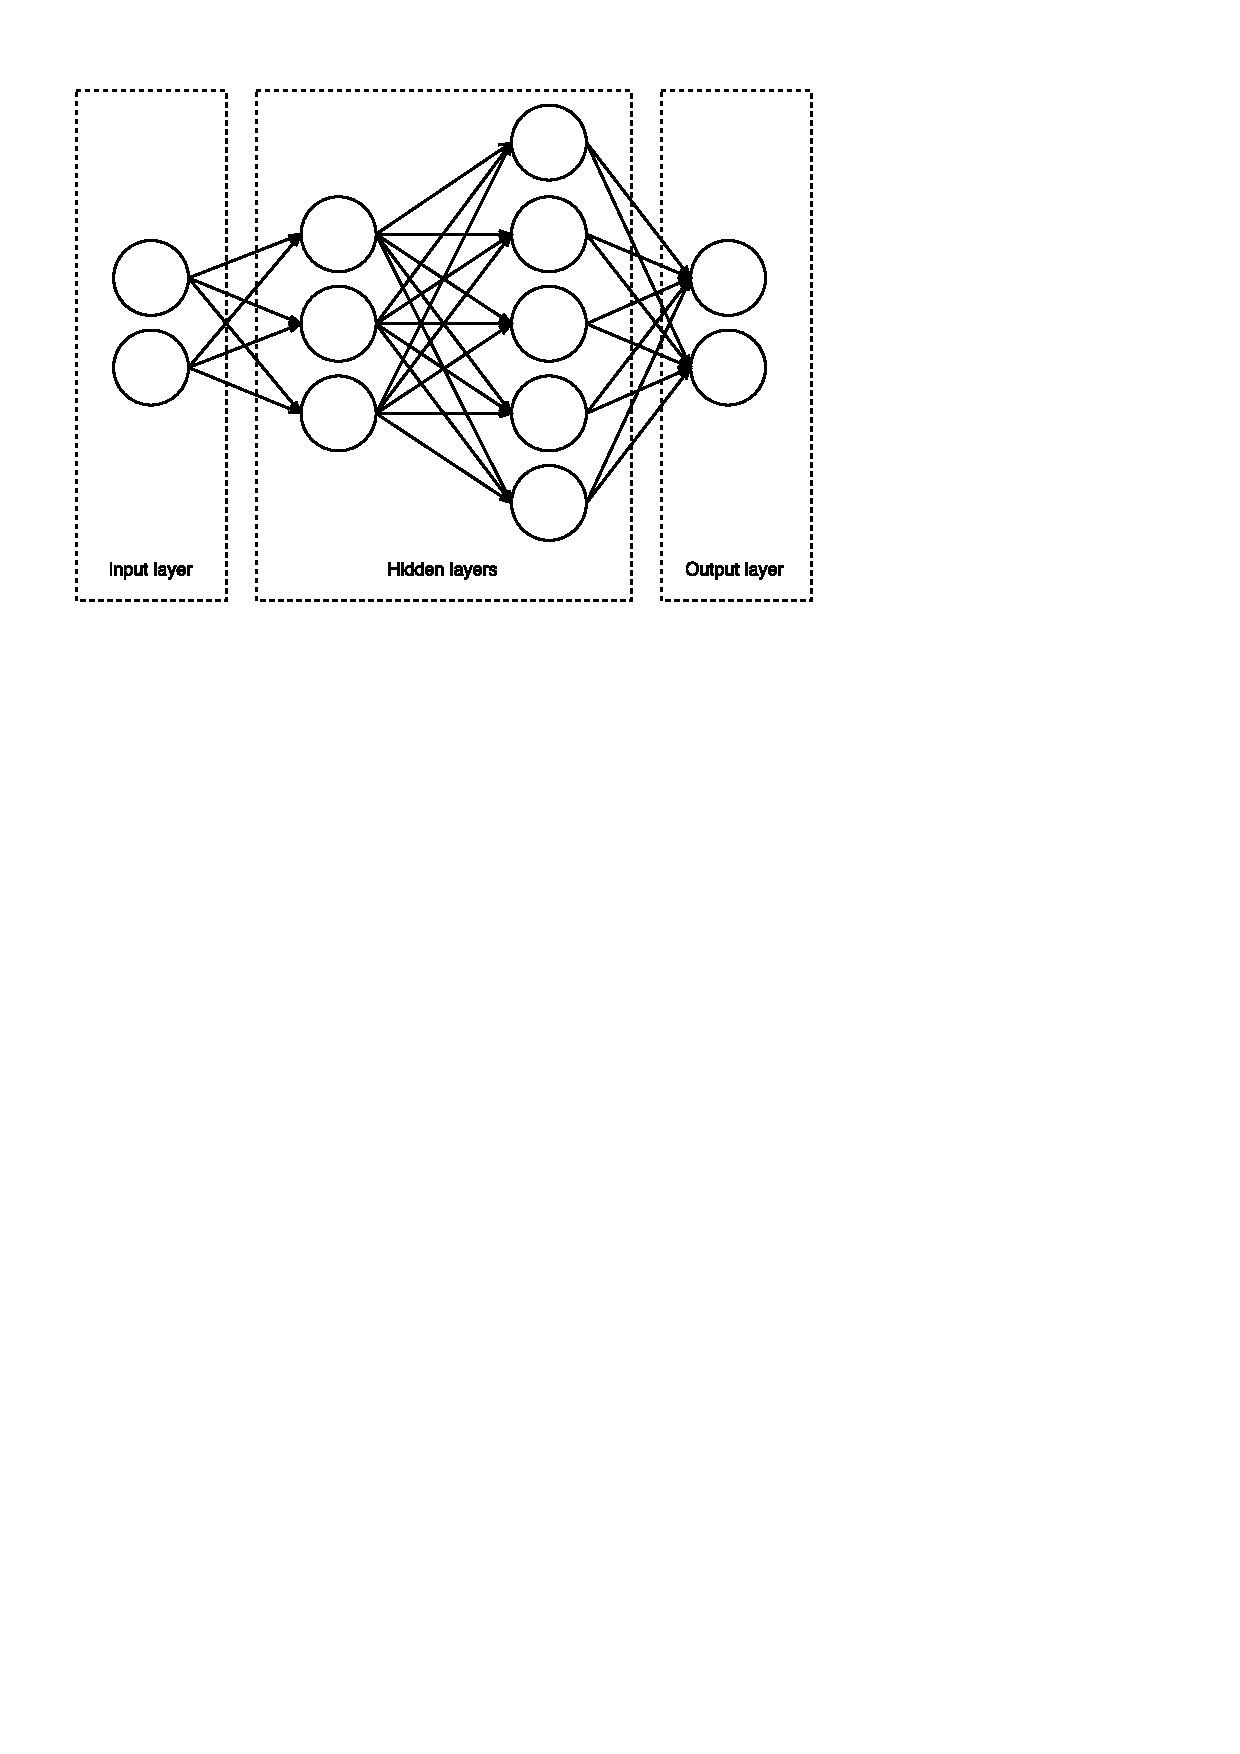
\includegraphics[scale=0.6]{nn_layout}
	\caption{Structure of a simple neural network with two hidden layers.}
	\label{fig:nn_layout}
\end{figure}

Each neuron in layer $n+1$ is connected to every neuron in layer $n$ and computes as an output
\[y = f_{act}((\sum_{i=1}^{n} y_i w_i) + b)\]
where $f_{act}$ is a non-linear, differentiable activation function and $y_i$ is the output of neuron $i$ in the previous layer. A neuron is connected to every neuron in the previous layer, which is why this layer is also referred to as a fully connected layer.
\subsubsection{Activation functions}
The most common activation functions are the Sigmoid function,
\[S(x) = \frac{1}{1 + e^x}\] the hyperbolic tangent 
\[\textrm{tanh}(x)=\frac{e^x - e^{-x}}{e^x + e^{-x}}\] the rectifier 
\[
f(x) = 
\begin{cases}
	0 & \text{if } x < 0\\
	x & \text{otherwise}
\end{cases}
\]
and the leaky rectifier, for some $0 < \alpha < 1$
\[
f(x) = 
\begin{cases}
	\alpha x & \text{if } x < 0\\
	x & \text{otherwise}
\end{cases}
\]
This functions can be seen plotted in figure \ref{fig:activation_functions}. 
\begin{figure}
	\centering
	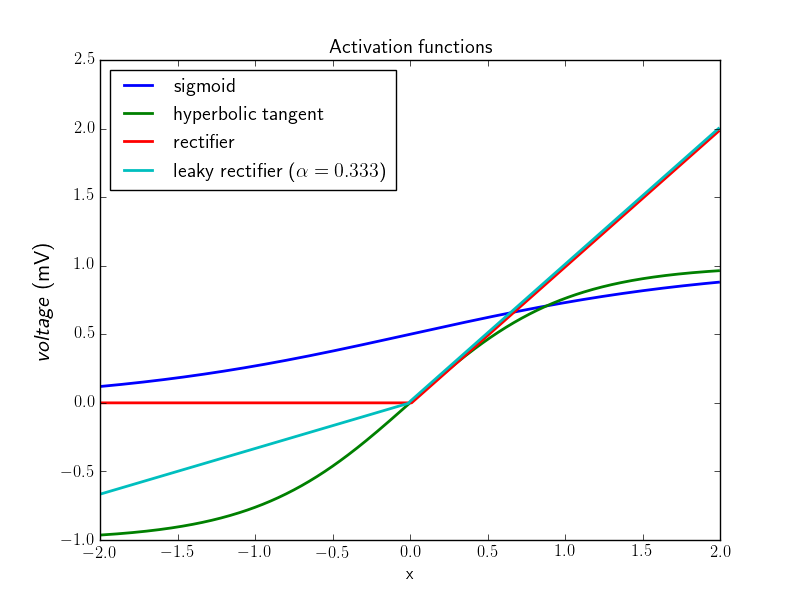
\includegraphics[scale=0.6]{activations}
	\caption{Plot of the activation functions.}
	\label{fig:activation_functions}
\end{figure}
Historically, the hyperbolic tangent function or the sigmoid function have been used as activation functions. However, as the magnitude of the gradients of those functions is always below 1, these activation function create a problem of vanishing gradients for deeper networks, as we have to multiply those gradients together for each layer. [CITATIONS!!!!] This is why it is nowadays preferred to use the rectifier or the leaky rectifier functions, especially with deeper architectures.

In a classification problem, the output layer will consist of $K$ nodes, one for each class. Using a softmax activation function for the last layer, we can view the output of node $k$ as the probability $P(y^{(i)} = k \mid \mathbf{x}^{(i)};\theta)$ since the the output of each neuron will range between 0 and 1 and the sum of all outputs will be 1. The softmax activation computes for each output $k$
\begin{equation}
	\sigma(\mathbf{x})_k = \frac{e^{\mathbf{x}_k}}{\sum_{j=1}^{K}e^{\mathbf{x}_j}}
\end{equation}
where $\mathbf{x}$ is the vector consisting of all outputs from the previous layer.

\subsubsection{Loss function}
The next step is to compute how well our network approximates our training data with a loss function, to then decide how to change the weights of the network in order to minimise the loss. Since the aim of the network is to classify the central pixel(s) of the patch, we use the categorical cross-entropy loss function
\begin{equation}
	\label{eq:loss}
	\mathcal{L}(\theta) = 
	\frac{1}{m}\Big[\sum_{i=1}^m \sum_{j=1}^k\mathbbm{1}[y^{(i)} = k]\log(P(y^{(i)}=k \mid \mathbf{x}^{(i)};\theta))\Big]
\end{equation}
where $\mathbbm{1}$ is the indicator function and $P(y^{(i)}=k \mid \mathbf{x}^{(i)};\theta)$ is the probability computed by the neural network that input vector $\mathbf{x}$, in our case a patch, belongs to class $k$.

\subsubsection{Optimisation}
The next step is to calculate the gradient $\dfrac{d\mathcal{L}(\theta)}{d\theta}$, so that we can apply gradient descent and update our weight vector to
\begin{equation}
	\theta = \theta - \epsilon \frac{d\mathcal{L}(\theta)}{d\theta}
\end{equation}
where $\epsilon$ is the learning rate, a small positive value.

Since every basic operation used in the neural network is differentiable, the entire network will also be differentiable, which in turn makes it possible to calculate the gradient of a loss function with respect to the weights in the network. This process is called backpropagation.

The loss functions, as described in equation \ref{eq:loss} is computed using the entire training data set $\mathbb{X} = \{(\mathbf{x}^{(1)},y^{(1)}), ...,(\mathbf{x}^{(m)},y^{(m)})\}$. In the case of deep learning where it is usual to have a very large training data set, this would be very memory costly and slow down the training phase unnecessarily. Therefore, stochastic gradient descent is used instead, where we process the training data sequentially in batches, each time computing the loss for that batch and updating the weights.

\subsubsection{Momentum}
A further optimisation used to speed up the training process is momentum update. Minimising the loss function can be interpreted as moving a small particle down a hilly terrain in the hyper-dimensional space defined by the loss function. Since the gradient is related to the force experienced by that particle, this suggest that the gradient should only influence the velocity vector and not the position directly. This leads to the velocity update
\begin{equation}
	v = \mu  v - \epsilon \frac{d\mathcal{L}(\theta)}{d\theta}
\end{equation}
where $\mu$ is the momentum, typically set to 0.9. We then update our weights by simply adding the velocity to the current value.
\begin{equation}
	\theta = \theta + v
\end{equation}

Typically a slightly different version, called the Nesterov momentum, is used as it has been shown to work better in practice[CITATION].

\subsubsection{Further optimizations}
Should I explain adam optimisation??

\subsection{Convolutional neural networks}
Convolutional neural networks are different as they make the explicit assumption that the inputs will be images. This allows us to take advantage of some properties to make the forward function more effective and greatly reduce the number of weights in our network. 

A typical convolutional network constists of three types of layers: \textbf{convolutional layers}, \textbf{pooling layers} and \textbf{fully-connected layers}. 
\subsubsection{Fully-connected layers}
These are exactly the same as for ordinary neural networks.

\subsubsection{Convolutional layers}
Unlike a fully-connected layer, a convolutional layer is typically three-dimensional: widht, height and depth. The parameters of a layer are a set of learnable filters, each spatially small along the width and height but with the depth equal to the depth of input volume. The layer then computes a two-dimensional activation map by convolving the filter with the input and computing the dot product at each point. This means that the function learned by a filter has translational invariance, as the filter is convolved with the entire input and thus the same feature is detected independently of location. Each filter computes such a two-dimensional activation map that can then be stacked along the depth axis to produce the output volume.

The connectivity pattern is inspired by the organization of the animal visual cortex. Individual neurons respond to stimuli in a small region of space known as the \textbf{receptive field}. Every element in the output can then be interpreted as the output of a neuron whose receptive field is the width and height of the filter and who shares its weights with all its neighbours to the left and right spatially.

The size of the output volume is determined by three hyperparameters.
\begin{enumerate}
	\item The \textbf{depth} corresponds to the number of filters in the layer and is therefore equal to the depth of the output volume.
	\item The \textbf{stride} which determines by how many pixels we slide the filter. When the stride is greater than 1 the output width and height will be smaller than the input width and height.
	\item The \textbf{padding} determines with how many zeros we pad the input width and height. This is particularly useful when we want to preserve the input dimensions.
\end{enumerate}
The computation done by such a filter in shown in figure \ref{fig:conv_example}.

\begin{figure}[h]
	\centering
	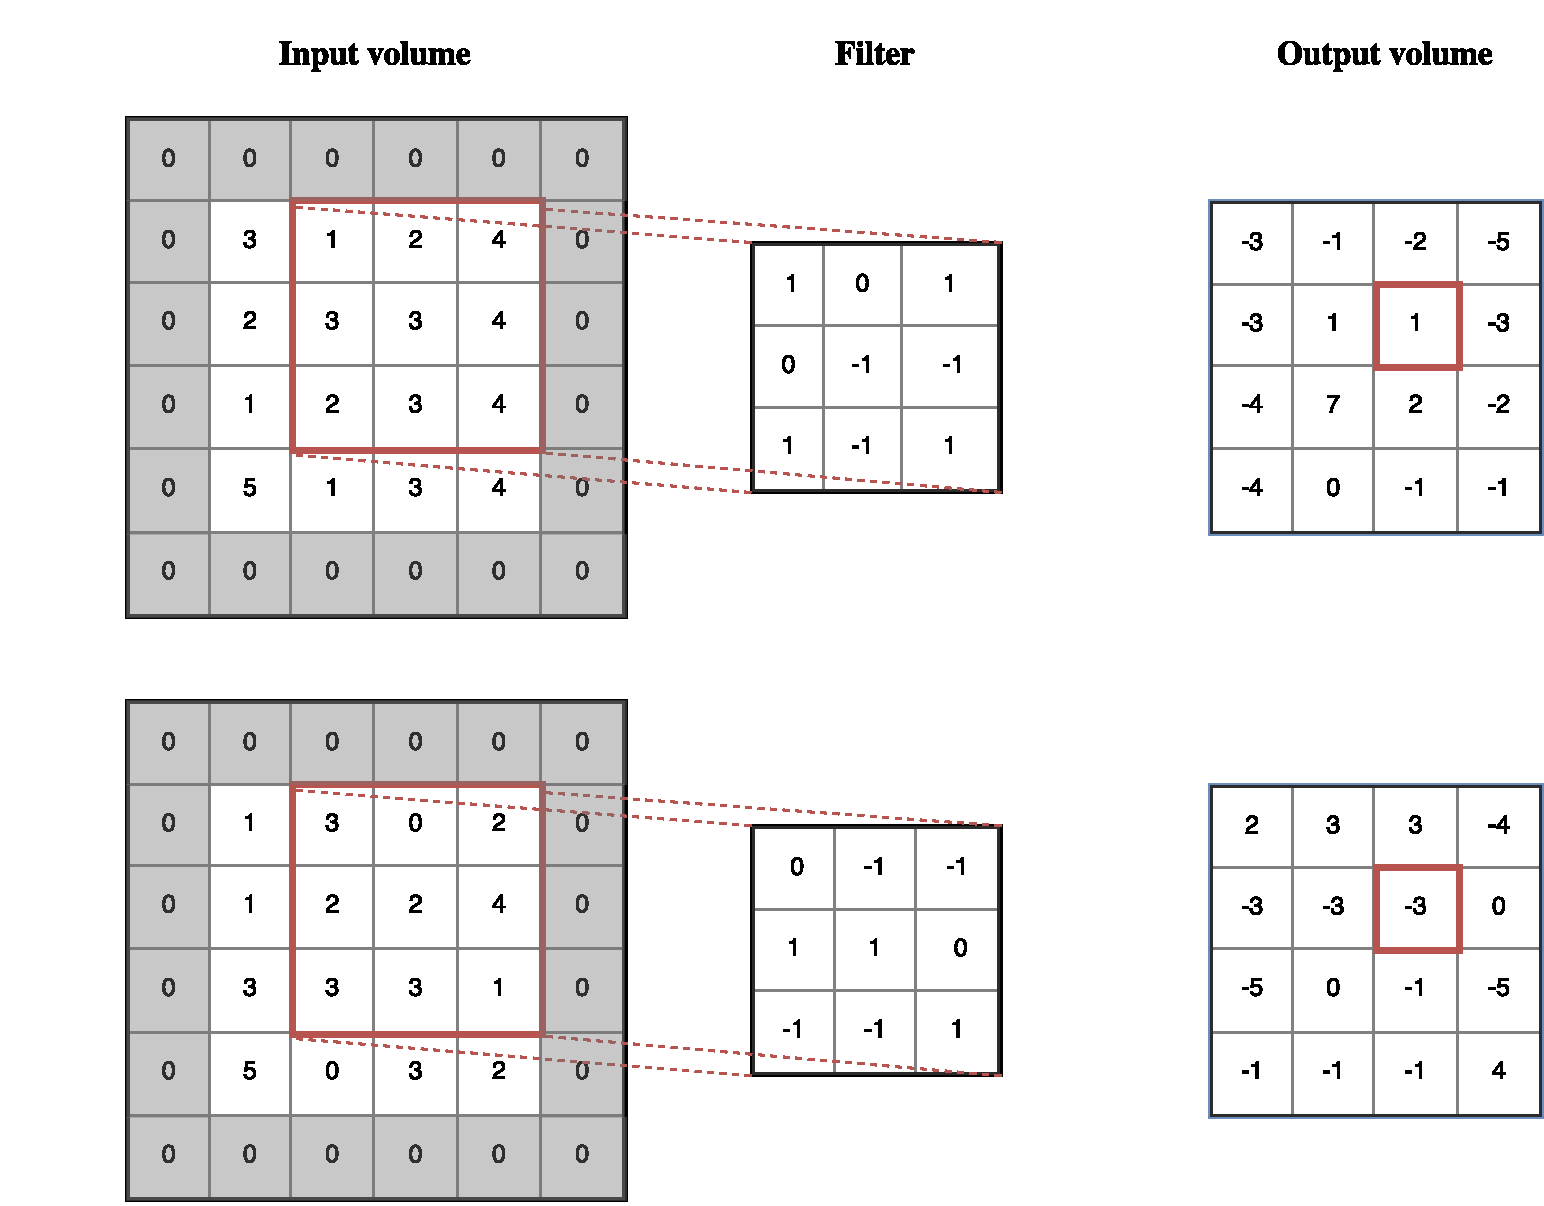
\includegraphics[scale=0.6]{conv_example}
	\caption[Example computation done by a 3x3 filter in a convolutional layer]{Example computation done by a 3x3 filter in a convolutional layer. Both the stride and the padding are 1, so as to keep the output dimensions identical. The output at depth 0 for the marked element is $1 \cdot 1 + 2 \cdot 0 + 4 \cdot 1 + 3 \cdot 0 + 3 \cdot -1 + 4 \cdot -1 + 2 \cdot 1 + 3 \cdot -1 + 4 \cdot 1 = 1$ and similarly at depth 1 the output for that element is -3.}
	\label{fig:conv_example}
\end{figure}

\subsubsection{Pooling layers}
The function of the pooling layer is to reduce the spatial size of the input layer in order to reduce the number of parameters and computation in the network. The most common pooling layer implementation is the \textbf{max-pooling} which just convolves a two-dimensional maximum operator of a given size, typically 2x2. The \textbf{stride} again determines the step size.
\newline

A convolutional neural network typically consists of a sequence of these layers, starting with pairs of convolutional neural networks and max pooling layers. The idea behind this is that each pair of layers can learn more and more abstract features using the features learned by the previous layer. For example, the first pair might learn to recognise edges, the second layer shapes, etc.. The last few layers of the network consist entirely of fully-connected layers. These learn how to classify the data using the features learned by the convolutional and max pooling layers.

\subsection{The overfitting problem}
A common problem to arise in neural networks is that of \textbf{overfitting}, that is when the model isn't able to generalise on previously unseen data and instead just memorises the training data. Due to the large number of weights in convolutional neural networks, these are particularly prone to this problem. Many techniques and heuristics have been developed in order to help reduce overfitting. In particular, I used three of them: \textbf{L2 weight normalisation}, \textbf{Dropout} and \textbf{Batch Normalisation}
\subsubsection{\textbf{L2} weight normalisation}
The intuition behind this normalisation is that by preventing individual parameters to grow without bounds, the model must learn how to smoothly extract features of the data and this in turn will prevent the model from just memorising the data. This is achieved by adding a regularisation penalty to the loss function. The L2 normalisation computes the sum of the squares of every parameter:
\begin{equation}
	R(\theta) = \sum_{k}^{} \sum_{l}^{} \theta_{k,l}^2
\end{equation} 
Hence, the new loss function is
\begin{equation}
	\mathcal{L}(\theta) = \mathcal{L}_{data}(\theta) + R(\theta) 
\end{equation}
where $\mathcal{L}_{data}(\theta)$ is the data loss, defined in equation \ref{eq:loss}. 
Although I have only used the L2 normalisation (explain why?), it is important to realise that different regularisation penalties could be used, which lead to different regularisations.
\subsubsection{Dropout}
TODO
\subsubsection{Batch Normalisation}
TODO
\section{Data source}
\subsection{BraTS Challenge}
The dataset I am using comes entirely from the BraTS \cite{menze:hal-00935640} challenge. It is split into three sections:
\begin{enumerate}
	\item The training dataset, which consists of 30 different patients and their ground truth marked by a human experts. The 30 patients are further divided into 20 high-grade glioma cases (HG) and 10 low-grade glioma cases (LG). The difference between these two types of brain tumours is their rate  of growth, which is slower for the low-grade case.
	\item The challenge set, which consists of 10 high-grade patients without the ground truth. These scans are meant to be segmented by the participants of the challenge, who can then submit their segmentation online. 	
	\item The leaderboard set contains 25 patients, including both high-grade and low-grade gliomas. The ground truth labels are not available.
\end{enumerate}
The challenge and leaderboard sets were both used to rank the participants of the original BraTS conference. After the conference, to create a benchmarking resource, an online platform was made available that automatically calculates the scores (Dice score, PPV and Sensitivity) of submitted segmentations. Part of the evaluation of my project will be comparing the results of my model with those made by other researchers using this online platform.

Each patient consists of 4 images taken using different MRI contrasts: T2 and FLAIR MRI which highlight differences in tissue water relaxational properties, T1 MRI which shows pathological intratumoral take-up of contrast agents and T1c MRI. Each of these modalities shows different type of biological information and may therefore be useful for creating different features during the classification of the tissues.
Figure \ref{fig:mri_scans} shows the 4 different modalities for a slice in the axial plane for a patient. 
\begin{figure}[h]
	\centering
	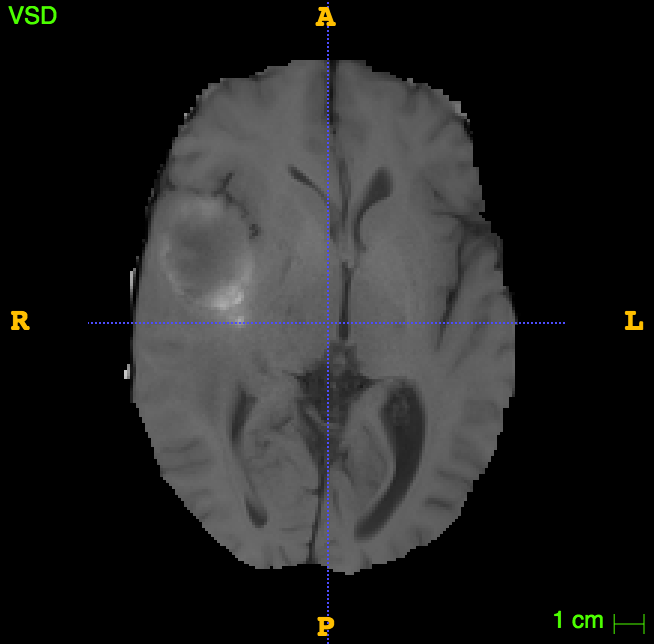
\includegraphics[scale=0.15]{T1_example}
	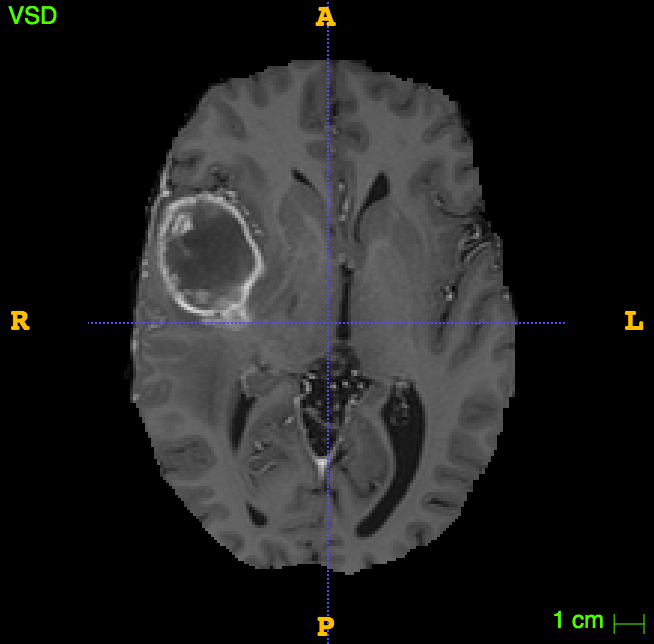
\includegraphics[scale=0.15]{T1c_example}
	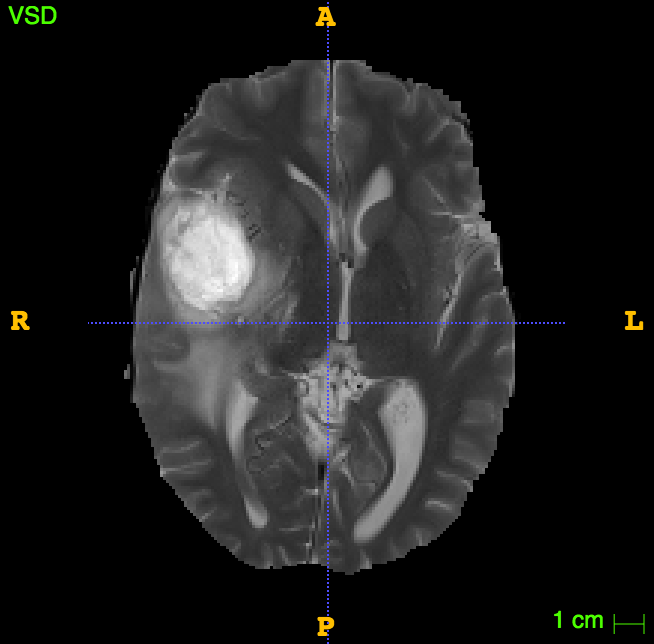
\includegraphics[scale=0.15]{T2_example}			
	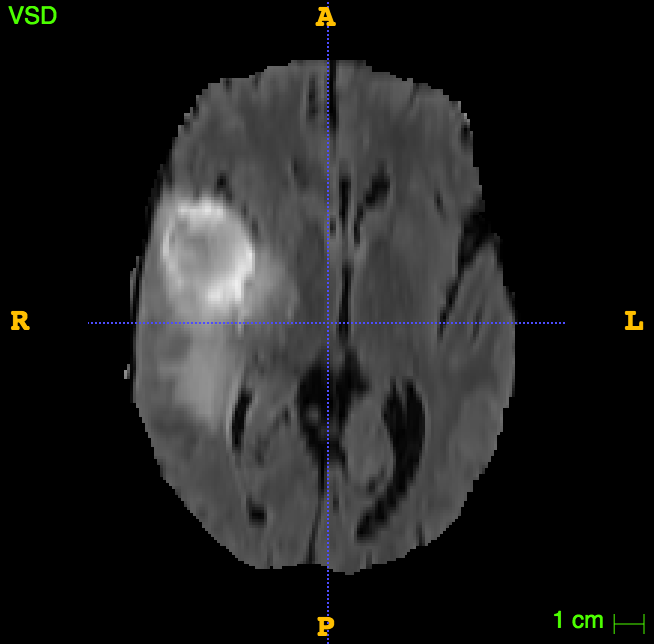
\includegraphics[scale=0.15]{Flair_example}
	\caption[Example slices in the axial plane for the 4 different scan modalities]{Example slices in the axial plane for the 4 different scan modalities. From left to right the modalities are T1, T1c, T2 and Flair. The scan is from patient 1, slice $z=89$. The four modalities have some obvious differences which the convolutional neural network might be able to utilise to discriminate between tumour and non-tumour regions.}
	\label{fig:mri_scans}
\end{figure}
Figure \ref{fig:expert_segmentations} shows different slices of a T1 MRI scan annotated with the ground truth labelling created by a group of 4 experts.
\begin{figure}[h]
	\centering
	\includegraphics[scale=0.1]{expert_segmentation_49}
	\includegraphics[scale=0.1]{expert_segmentation_59}
	\includegraphics[scale=0.1]{expert_segmentation_69}
	\includegraphics[scale=0.1]{expert_segmentation_79}
	\includegraphics[scale=0.1]{expert_segmentation_89}
	\includegraphics[scale=0.1]{expert_segmentation_99}
	\includegraphics[scale=0.1]{expert_segmentation_109}
	\includegraphics[scale=0.1]{expert_segmentation_119}
	\includegraphics[scale=0.1]{expert_segmentation_129}
	\caption[Slices of a T1 MRI scan annotated with the expert labelling.]{Axial plane slices of a T1 MRI scan annotated by the expert labelling. The slices were taken from patient 1, using $z \in \{49, 59, 69, 79, 89, 99, 109, 119, 129\}$. The enhancing tumour region is in yellow, the non-enhancing tumour in blue, the edema in green and the necrotic core in red, corresponding to classes 4, 3, 2 and 1 respectively.}
	\label{fig:mri_scans}
\end{figure}

To homogenise the data across the different scans, each patient's image volumes were co-registered to the T1c MRI scan, which has the highest spatial resolution in most cases. Then, all images were resampled to 1mm isotropic resolution in a standardised axial orientation with linear interpolation. Finally, all images were skull stripped to guarantee the anonymity of the patients.


\subsection{Data used in this project}
For this project I have decided to focus only on the high-grade glioma cases. This decision was mainly made to keep the scope of this project reasonable. Secondly, the results of most research papers in this area are commonly reported in terms of high-grade glioma cases as it is considered to be harder than the low-grade cases. Lastly, the challenge dataset, which consists only of high-grade patients allowed me to compare easily the results of my models with those of other researchers. Thus only the 20 high-grade glioma cases of the training dataset were used as training data. 

To provide some guidance on how well the network is performing during the training phase, I also used 10 high-grade glioma cases from the BraTS2015 dataset, which contains more patients prepared in a similar way. These 10 patients were used to provide the validation data.

\chapter{Implementation [40\%]}

\section{Data pre-processing}
The first step is to read in the scans, which is done using the SimpleITK library that has inbuilt support for the MetaImage medical (`.mha') format. For each patient the 4 scans (T1, T1c, T2, Flair) are read in as numpy arrays and stacked along a new dimension, resulting in a 4-dimensional array for each patient of shape $(z_{\text{size}} \times y_{\text{size}} \times x_{\text{size}} \times 4)$. I then aggregate those arrays into a single conveniently-formatted list containing all the training data.

\subsection{Patch extraction}
Each input to the neural network is a three-dimensional array, of shape $33 \times 33 \times 4$, since it consists of a two-dimensional patch of $33 \times 33$ voxels for each one of the 4 scan modalities. The two-dimensional patches are taken along the x--y axis, refer to as the axial plane in anatomy. Figure \ref{fig:patch_extraction} gives an overview of this process.

\begin{figure}
	\centering
	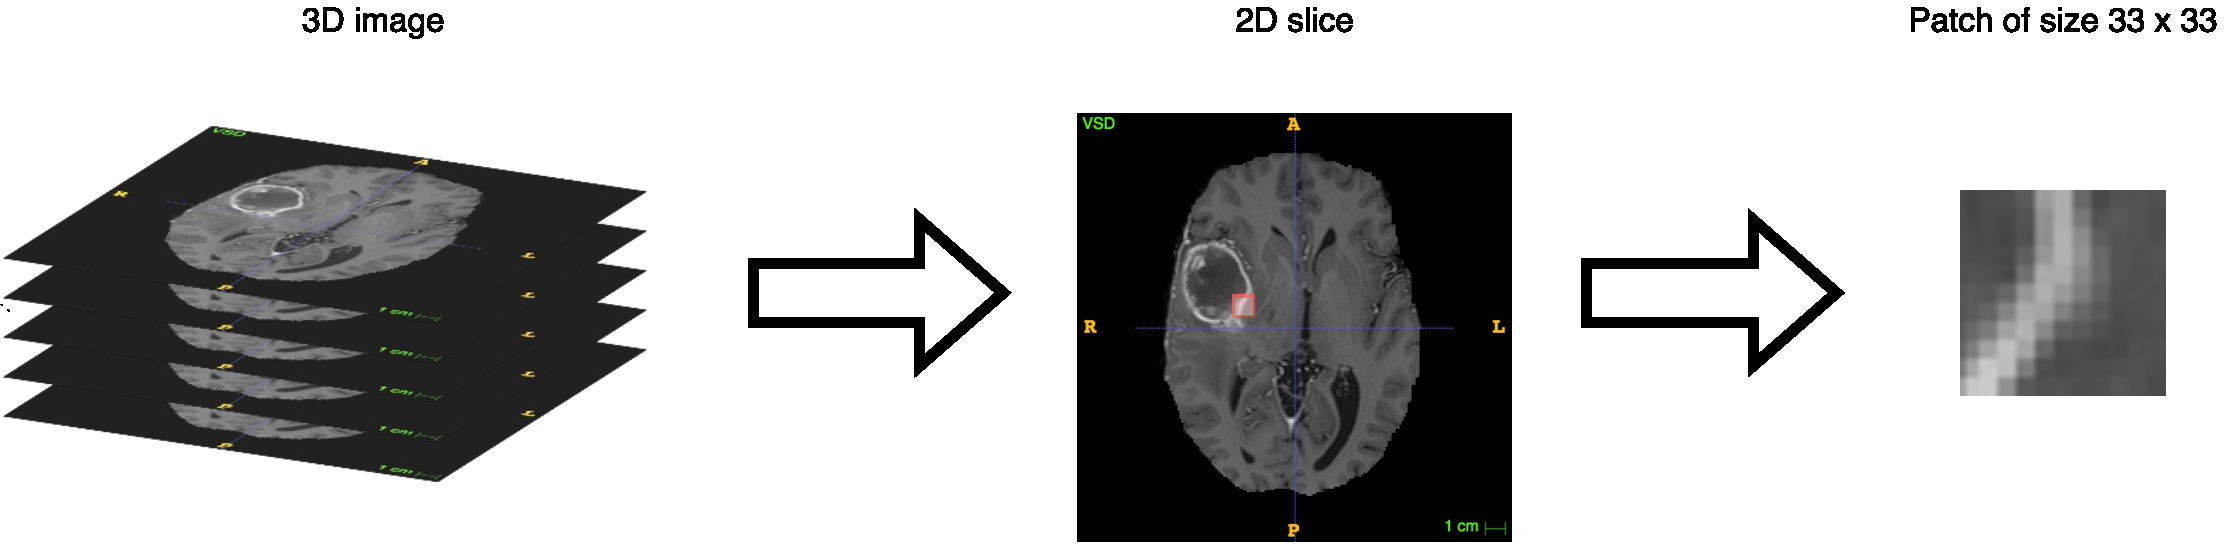
\includegraphics[scale=0.43]{patch_extraction}
	\caption{Convolutional network architecture proposed by Pereira et al.}
	\label{fig:patch_extraction}
\end{figure}

 
As explained in the previous chapter the data consists of 20 different patients, each consisting of 4 different MRI scans, taken with different modalities. Unfortunately, the size of the different scans varies from patient to patient. Table \ref{table:scan_sizes} shows how the sizes are distributed among patients. Since we are working with individual patches, this discrepancy in scans sizes between patients has no impact, as long as each voxel has the same spatial resolution. This can be seen as one of the advantages of a model based on patches compared to a model based on slices or even entire MRI scans, as it offers more flexibility on the size of the MRI scans.

\begin{table}[h]
\centering	
\label{table:scan_sizes}
\begin{tabular}{ c c } 
\textbf{Size} & \textbf{Number of scans}\\
 \hline
 $\ 176 \times 216 \times 160$ & 8 \\ 
 $\ 176 \times 216 \times 176$ & 6 \\ 
 $\ 230 \times 230 \times 162$ & 2 \\ 
 $\ 176 \times 236 \times 216$ & 1 \\ 
 $\ 165 \times 230 \times 230$ & 1 \\ 
 $\ 240 \times 240 \times 168$ & 1 \\ 
 $\ 220 \times 220 \times 168$ & 1 \\ 

\end{tabular}
\caption{Scan sizes in voxels for the 20 different patients, dimensions are ordered as $(z \times y \times z)$}
\end{table}

The dataset used is also extremely unbalanced, which would cause issues if the model was training using patches chosen uniformly at random from the scans. Table \ref{table:class_frequencies} shows the proportion of data available in each class. Because the training data for the convolutional neural network should be balanced, we need to extract the same number of patches for each class. Note that this further implies that the maximum number of patches we can extract is 5 times the number of voxels in the least represented class, which is the non-enhancing tumour class with 184,436 labeled voxels, for a maximum of 922,130 of patches.

\begin{table}
\centering	
\label{table:class_frequencies}
\begin{tabular}{c c S[table-format=9.0] S[table-format=2.2]}
\textbf{Class} & \textbf{Tissue type} & \textbf{Number of labeled voxels} & \textbf{frequency}\\
 \hline
0 & Non tumour 				& 138958832 	& 98.23 \% \\ 
1 & Necrosis 				& 282936 	& 0.20 \% \\ 
2 & Edema					& 1466271 	& 1.36 \% \\ 
3 & Non-enhancing tumour 	& 184436 	& 0.13 \% \\ 
4 & Enhancing tumour		& 560777 	& 0.34 \% \\

\end{tabular}
\caption{Class frequencies in the BraTS2013 HG dataset. The normal tissue (class 0) is highly overrepresented, which leads to issues when training the convolutional neural network. We therefore have to balance the dataset when extracting the patches.}
\end{table}

A further question is how we should deal with a voxel that is to close to the edge of the scan to be able to extract an entire patch around it. I could either ignore the patch or pad the scan such that each labelled voxel is surrounded by enough voxels. The first option is not only easier, but also helps with the balanced classes issue as most of the voxels close to an edge are from class 0. This is because the brains are centered within the scans. Table \ref{table:valid_class_frequencies} shows the distribution of classes for ``valid'' voxels, .i.e those at least more than half the patch length away from the x or y edges.
\begin{table}[h]
\centering	
\label{table:valid_class_frequencies}
\begin{tabular}{c c S[table-format=9.0] S[table-format=2.2] S[table-format=8.0]}
\textbf{Class} & \textbf{Tissue type} & \textbf{Labelled voxels} & \textbf{Frequency} & \textbf{Ignored voxels}\\
 \hline
0 & Non tumour 				& 94773429 	& 97.45 \% & 44185403 \\ 
1 & Necrosis 				& 281831 	& 0.29 \% & 1105\\ 
2 & Edema					& 1453205 	& 1.49 \% & 13066\\ 
3 & Non-enhancing tumour 	& 183396 	& 0.19 \% & 1040\\ 
4 & Enhancing tumour		& 558320 	& 0.57 \% & 2457\\

\end{tabular}
\caption{Class frequencies in the BraTS2013 HG dataset for valid voxels only, that is, those voxels it is possible to extract a patch of size $33 \times 33$ around. As most of the ignored voxels are in class 0, we can safely ignore them.}
\end{table}

The patch extraction can now be performed. First I created a list for each class containing the positions of the valid voxels for that class. Note that at this point it would be unfeasible to store the patches, as it would require to store over a 100 billion 32 bit floats for class 0 alone, or over 400 GB. To get the indices of the valid voxels, I used numpy's argwhere function on the ground truth arrays. The argwhere function takes in an array and a predicate and returns the indices of those elements in the array satisfying the predicate. Here, the predicate used is just equality checking between the voxel label and the class number. This is done for every patient. Since the scan number must also be included in the indices, I prepended the scan number along the first axis, before aggregating the results for each patient into a list. The final result is a list for each class that contains tuples of the form $(\text{patient number}, z, y, x)$. The second step consists of removing those voxels that are too close to an x-axis or y-axis edge. Only indices $(\text{patient}, z, y, x)$ where the x and y values are  within the allowed ranges of $[16, \text{size}-(16+1)]$ are kept. Again this can be done using numpy and filtering based on column values. Algorithm \ref{alg:patch_extraction} summarises the steps taken during the patch extraction.

\begin{algorithm}[h]
\caption{Patch extraction}\label{alg:patch_extraction}
\begin{algorithmic}[1]
\For{$\text{class } k \text{ in } [0,1,2,3,4]$}
	\State valid\_indices[$k$] $\gets$ []
	\For{\textbf{each} index, label \textbf{in} labels} 
		\State possible\_indices $\gets$ \textit{numpy}.argwhere($label == k$)
		\State patient\_indices $\gets$ \textit{numpy}.full(\textit{len}(possible\_indices), index)
		\State possible\_indices $\gets$ \textit{numpy}.append(patient\_indices, possible\_indices, axis = 1)
		\State
		\State possible\_indices $\gets$ possible\_indices[$\text{possible\_indices}[:,2] - 16 \ge 0$]
		\State possible\_indices $\gets$ possible\_indices[$\text{possible\_indices}[:,2] + (16+1) < $ label.y\_dimension]
		\State possible\_indices $\gets$ possible\_indices[$\text{possible\_indices}[:,3] - 16 \ge 0$]
		\State possible\_indices $\gets$ possible\_indices[$\text{possible\_indices}[:,3] + (16+1) < $ label.x\_dimension]
		\State
		\State valid\_indices[$k$] $\gets$ possible\_indices
	\EndFor
\EndFor
\end{algorithmic}
\end{algorithm}

\subsection{Data augmentation}
To increase the amount of data available, some data augmentation techniques can be used. In typical applications of convolutional neural networks for image processing and computer vision tasks, translation and rotations can be used. Since the data consists entirely of two-dimensional patches, translation is useless as it would just result in a different patch, with a possibly different label. However, using rotations of the patches might give some performance improvements. Pereira et al. proposes different techniques in \cite{pereira}:
\begin{enumerate}
	\item No rotations
	\item Rotations of 0, 90, 180 and 270 degrees.
	\item Rotations of multiples (???)
\end{enumerate}
Using rotations of multiples of 90 degrees performed the best, which is why I have decided to perform those. I also have investigate the effect on the results of using no rotations at all, the results are reported in the evaluation chapter (MAYBE).

Once again, Keras is extremely useful as it allows the creation of ``ImageDataGenerators'' which given two numpy arrays of the training data and labels, generates batches of augmented data in real-time during the training phase of the convolutional neural network. In particular it is possible to randomly flip the images vertically and horizontally, which was used to `rotate' the images.

Note that, as opposed to the patch extraction and the normalisation phases, the data augmentation is only done for the training data and not for the validation or test data.

\subsection{Normalisations}
This section should explain what the next 3 normalisations do and how they are implemented, i.e. using python's numpy.
\subsubsection{Winsorising}
The first normalisation that is applied is called `winsorising'. The aim is to limit the values of extremes, in order to reduce the effect that outliers may have. This is also known as `clipping' in digital signal processing. I used a 98\% winsorisation, meaning that the data values below the 1\textsuperscript{st} percentile are set to the value of the 1\textsuperscript{st} percentile and the value above the 99\textsuperscript{th} percentile are set to the value of the 99\textsuperscript{th} percentile. Note that this process is different from trimming as the values are not discarded but just modified.
\subsubsection{N4ITK}
This section might be slightly longer. It should definitely include a picture of a comparison of some slices before and after the normalisation. I am not sure if I should explain what the normalisation actually does as it is quite complicated.

\subsubsection{Linear scaling}
Then, each scan with different modality is individually scaled into the range $[0,1]$. This is done to guarantee that the absolute values of the different scans are within the same range, making it possibly easier for the convolutional neural network to generalise the features it learns onto new data. In general to linearly scale a data point $x$ into the range $[a, b]$, the formula described in equation \ref{eq:linear_scaling_general} is applied, where $x_{min}$ and $x_{max}$ are the minimum and maximum value across the dataset to scale.
\begin{equation}
	\label{eq:linear_scaling_general}
	x' = a + (b - a)\frac{x - x_{min}}{x_{max} - x_{min}}
\end{equation}
Since, I am scaling to the range $[0,1]$ the formula becomes
\begin{equation}
	x' = \frac{x - x_{min}}{x_{max} - x_{min}}
\end{equation}
Using numpy's `min' and `max' function, we can perform this computation in a single line by using the fact that addition, subtraction and division is done element wise.

\subsubsection{Mean and Variance standardisation}
The last step is to standardise the mean and variance for each scan. This is done by first subtracting the mean across all scan values and then dividing by the standard deviation. 
\begin{equation}
	x' = \frac{x - \mu}{\sigma}
\end{equation}
As $E[aX] = a E[X]$ and $Var[cX] = c^2Var[X]$ it is easy to see that after this transformation the mean will be 0 and the standard deviation will be 1. Also note that as the true mean and standard deviation are not known, the sample mean and sample standard deviation are used. 

\section{Pereira model}

\subsection{Architecture}

The model proposed by Pereira et al. \cite{pereira} consists of 11 layers, shown in figure \ref{fig:pereira_model}. 
\begin{figure}
	\centering
	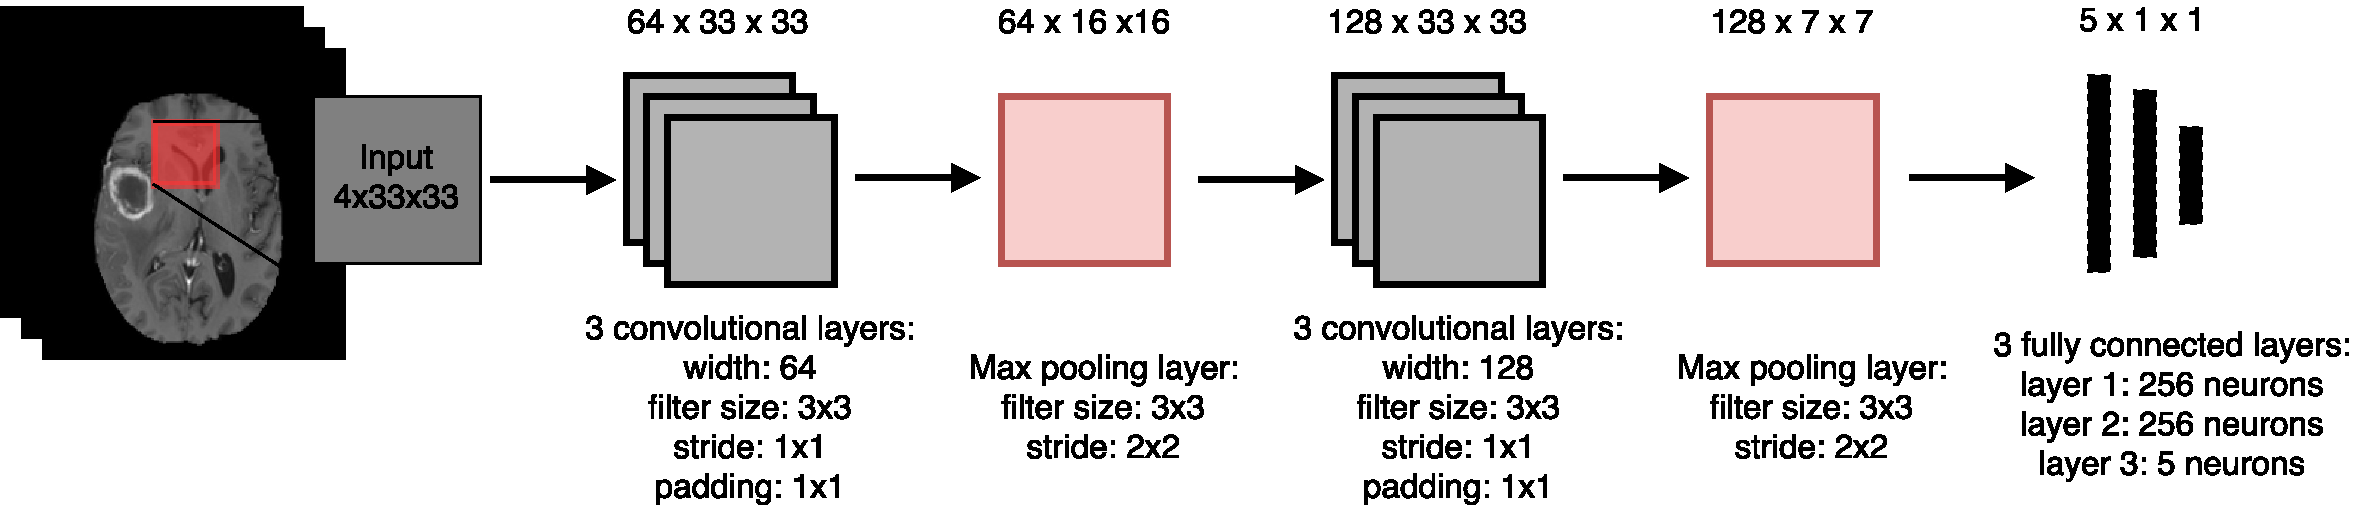
\includegraphics[scale=0.43]{pereira_model}
	\caption{Convolutional network architecture proposed by Pereire et al.}
	\label{fig:pereira_model}
\end{figure}
The first three layers are convolutional layers with filter size 3x3, stride 1x1 and width 64. Three layers are used consecutively because the combination of them  effectively has a receptive field of size 7x7 while having fewer parameters then a single 7x7 convolutional layer would have, making the network less prone to overfitting. [CITATION 36 in pereira]. The next layer is a max pooling layer of size 3x3 and stride 2x2. This is an unusual design as the size is larger than the stride. This is done because although pooling can be positive to eliminate unwanted details and achieve invariance, it can also eliminate some of the important details. By keeping the size of the layer larger than the stride, the pooling will overlap which will allow the network to keep more information about location. Next, three convolutional layers are applied, this time doubling the width to 128 filters. Again a max pooling layer with the same parameters as the previous one is applied, before adding three fully connected layers of size 256, 256 and 5 respectively. Table \ref{table:pereira_weights} shows the number of weights in each layer. 

\begin{table}
\centering	
\label{table:pereira_weights}
\begin{tabular}{ c c S[table-format=7.0] } 
\textbf{Layer type} & \textbf{Output shape} & \textbf{\# Parameters} \\
 \hline
 Conv 		& $\ 64 	\times 33 	\times 33$ 	& 2368 \\ 
 Conv 		& $\ 64 	\times 33 	\times 33$ 	& 36928 \\ 
 Conv 		& $\ 64 	\times 33 	\times 33$	& 36928 \\ 
Max-Pool 	& $\ 64 	\times 16 	\times 16$ 	& 0\\
 Conv 		& $128 		 \times 16 	\times 16$	& 73856 \\ 
 Conv 		& $128 		\times 16 	\times 16$ 	& 147584 \\ 
 Conv 		& $128 		\times 16 	\times 16$ 	& 147584 \\ 
Max-Pool 	& $128 		\times\ 7 	\times\ 7$	& 0\\
FC			& $256 		\times\ 1 	\times\ 1$	& 1605888\\
FC			& $256 		\times\ 1 	\times\ 1$	& 65792\\
FC			& $\quad 5 	\times\ 1 	\times\ 1$ 	& 1285\\
\hhline{~~=}
\rule{0pt}{3ex}    
&& 2118213\\
\end{tabular}
\caption[Summary of the architecture proposed by Pereira, including the number of parameters in each layer.]{Summary of the architecture proposed by Pereira, including the number of parameters in each layer. The network has a total of 2,118,213 trainable parameters.}
\end{table}


The initialisation of the weights in the convolutional layers was done using the Xavier initialisation \cite{Xavier_ini}. The biases were initialised to the fixed constant value 0.1, except for the last layer.

The activation function used throughout the network is the leaky rectifier, with  $\alpha = 0.333$. However, using a leaky rectifier over a rectifier has very little effect on the final results, as will be shown in the next chapter. ???

To avoid overfitting Dropout \cite{} is used in the fully-connected layers, with probability $p=0.1$ of removing a node from the network.

\subsection{Implementation of the architecture in Keras}
Since the architecture is entirely sequential, I used the keras `sequential' model to implement it. The 'sequential' model makes it possible to create networks by adding layers to it sequentially, as the name suggests. The layers I had to use had available implementations, and therefore building the network itself was relatively straightforward. First, an instance a of model is created:
\begin{lstlisting}[language=Python]
	model = Sequential()
\end{lstlisting}
Then, layers can be added by calling the `add' member function of the model. For example to add a convolutional layer, we first create an instance of the `Convolution2D' class and then add it to the model:
\begin{lstlisting}[language=Python]
	conv = Convolution2D(nb_filters, size[0], size[1], border_mode='same', init='glorot_normal')
	model.add(conv)
\end{lstlisting}
Note that the library makes it easy to specify how the weights should be initialised, by setting the `init' argument. The `border\_mode' determines if padding should be added and how much. In our case we want the output of the layer to have the same size as the input. Max pooling layers and fully-connected layers can be added similarly.
In Keras, activation functions are treated in the same way as layers. Hence, to add a leaky rectifier, as called LReLU, we add an instance of the `LeakyReLU` class to the model:
\begin{lstlisting}[language=Python]
	alpha = 0.333
	LReLU = LeakyReLU(alpha)
	model.add(LReLU)
\end{lstlisting}
Adding Dropout is again done similarly:
\begin{lstlisting}[language=Python]
	p = 0.1
	model.add(Dropout(p))
\end{lstlisting}
As the last step before being able to train the model, we need to specify which loss function and which algorithm should be used to respectively specify and minimise the loss function. Again, keras makes this very simple:
\begin{lstlisting}[language=Python]
	sgd = SGD(lr = 3e-5, decay =0.0, momentum = 0.9, nesterov = True)
	model.compile(optimizer=sgd, loss='categorical_crossentropy', metrics=['accuracy']
\end{lstlisting}

\subsection{Training}
The paper specifies that the model was trained over 20 epochs, passing each patch through the network once per epoch. The optimisation algorithm used is a standard stochastic gradient descent algorithm with Nesterov momentum ($\mu = 0.9$). The learning rate should be linearly decreased from $3 \times 10^{-5}$ to $3 \times 10^{-7}$. Keras doesn't implement this functionality, so it has to be done manually. This can be done using algoritm \ref{alg:linear_decay}

\begin{algorithm}
\caption{Training the model with linearly decaying learning rate}\label{alg:linear_decay}
\begin{algorithmic}[1]
\For{$i \text{ from } 0 \text{ to } \text{nb\_epochs}-1$} 
	\State $\text{learning\_rate} \gets \text{start\_rate} + i \times \dfrac{\text{end\_rate} - \text{start\_rate} }{ \text{nb\_epochs} - 1 }$
	\State train\_model(nb\_epochs = 1, learning\_rate)
\EndFor
\end{algorithmic}
\end{algorithm}

At the end of each epoch the loss function is evaluated on the validation dat and the accuracy (equation \ref{eq:accuracy}) is computed. The loss and accuracy are then reported to the standard output. Figure \ref{fig:training_output} shows part the output of training a network for a few epochs.
\begin{equation}
	\label{eq:accuracy}
		\text{accuracy} = 
	\frac{1}{m}\Big[\sum_{i=1}^m\mathbbm{1}[y^{(i)} = \argmax{k}P(y^{(i)}=k)]\Big]
\end{equation}
\begin{figure}[h]
	\centering
	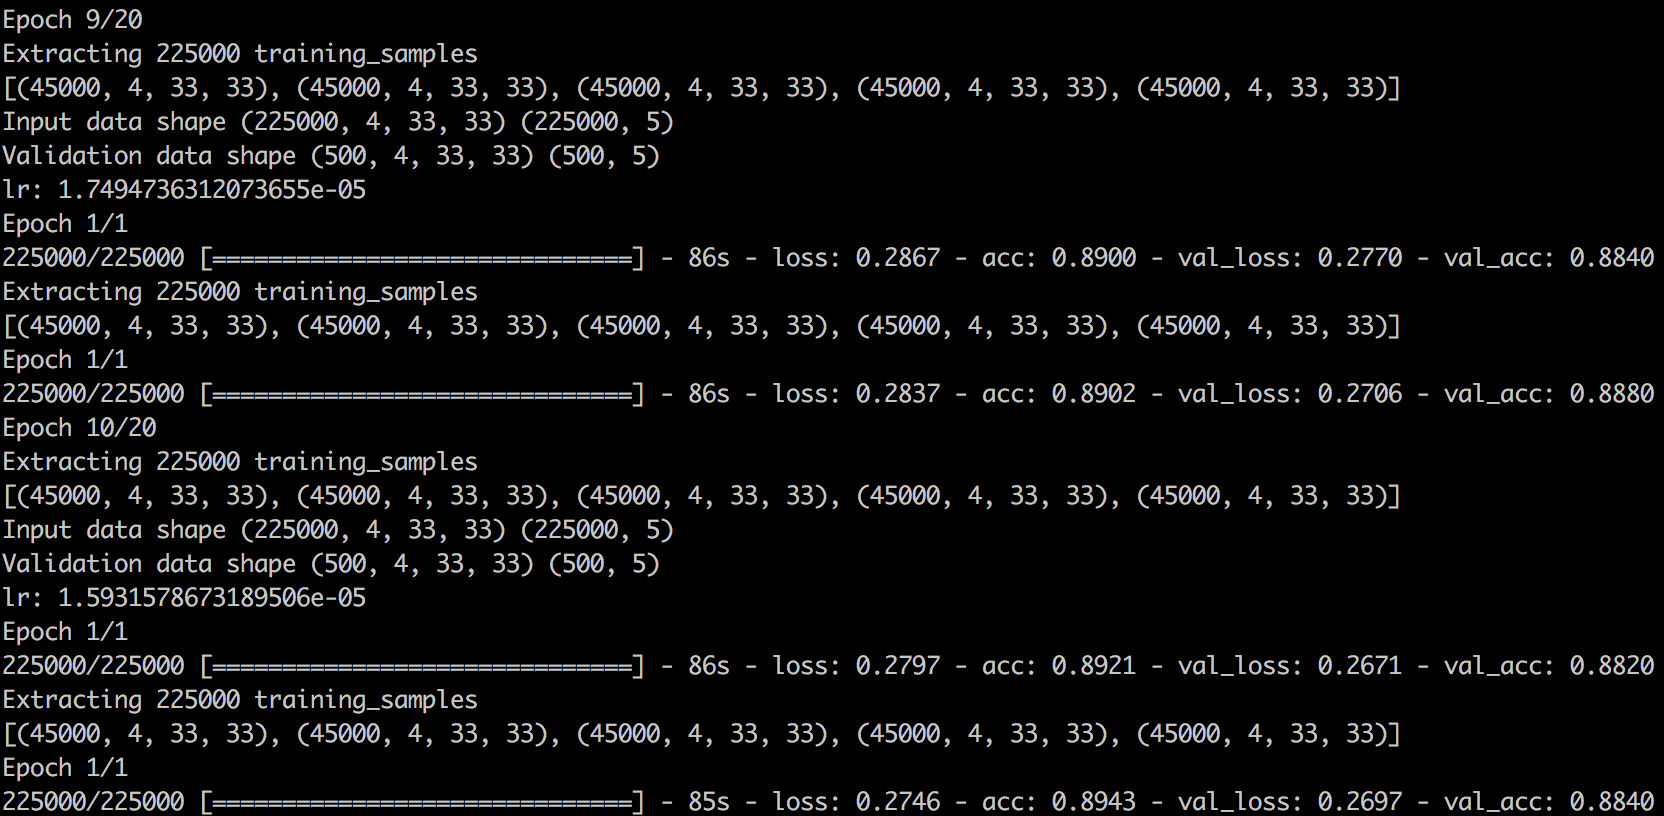
\includegraphics[width=\textwidth]{training_output}
	\caption[Part of the output of the training script]{Part of the of the training script. The output is shown for epochs 8 and 9. Both the validation loss and the validation accuracy are reported, as well as how long it took to train and validate for this epoch.}
	\label{fig:training_output}
\end{figure}

After training the model for 20 epochs, the model is saved in a directory specified as an argument to the main python script. Furthermore, to investigate how training the network for longer affects the results, each time the validation loss reaches a new minimum, the model at that point is also saved.

TODO: ADD GRAPH OF TRAINING/VALIDATION ACCURACY
\section{My model}
\subsection{Architecture}
\subsection{Implementation}
\subsection{Training}

\section{Segmentation}
\subsection{Pereira model}
\begin{enumerate}
	\item Explain how a scan is segemented 
	\begin{enumerate}
		\item  Normalising identically to the training data
		\item Adding 0 padding to the image to be able to classify all voxels
		\item 3 Convolve the model on the new bigger image.
	\end{enumerate}
\end{enumerate}
\subsection{My model}
\begin{enumerate}
	\item Similarly here, but show how it is more complicated as the model now predicts a single block of 64x1 voxels, which is really an 8x8 block and say that we want to use as large batch sizes as possible to accelerate the process.
\end{enumerate}

\section{Data post-processing}
\begin{enumerate}
	\item Explain how a connected components analysis is made to remove the small regions wrongly classified as a tumour region. Show an example of before and after.
\end{enumerate}
\chapter{Evaluation (+ Conclusion [20\%])}

\section{Metrics used for the evaluation}
\subsection{Regions of evaluation}
\subsection{Dice score}
\subsection{Positive predictive value}
\subsection{Sensitivity}

\section{Evaluation of the model proposed by Pereira et al.}
\section{Evaluation of my model}
\section{Comparison}

\chapter{Conclusion}
\section{Summary of achievements}
\section{Future Work}

I hope that this rough guide to writing a dissertation is \LaTeX\ has
been helpful and saved you time.


%%%%%%%%%%%%%%%%%%%%%%%%%%%%%%%%%%%%%%%%%%%%%%%%%%%%%%%%%%%%%%%%%%%%%
% the bibliography
\addcontentsline{toc}{chapter}{Bibliography}
\bibliography{refs}

%%%%%%%%%%%%%%%%%%%%%%%%%%%%%%%%%%%%%%%%%%%%%%%%%%%%%%%%%%%%%%%%%%%%%
% the appendices
%\appendix
%
%\chapter{Latex source}
%
%\section{diss.tex}
%{\scriptsize\verbatiminput{diss.tex}}
%
%%\section{proposal.tex}
%{\scriptsize\verbatiminput{proposal.tex}}
%
%\chapter{Makefile}
%
%\section{makefile}\label{makefile}
%{\scriptsize\verbatiminput{makefile.txt}}
%
%\section{refs.bib}
%{\scriptsize\verbatiminput{refs.bib}}
%
%
%\chapter{Project Proposal}
%
%%% Note: this file can be compiled on its own, but is also included by
% diss.tex (using the docmute.sty package to ignore the preamble)
\documentclass[12pt,a4paper,twoside]{article}
\usepackage[pdfborder={0 0 0}]{hyperref}
\usepackage[margin=25mm]{geometry}
\usepackage{graphicx}
\usepackage{parskip}
\begin{document}

\begin{center}
\Large
Computer Science Tripos -- Part II -- Project Proposal\\[4mm]
\LARGE
Brain tumour segmentation using Convolutional Neural Networks

\large
S.~Borgeaud~dit~Avocat, Fitzwilliam College

Originator: D.~Wang

11 October 2016
\end{center}

\vspace{5mm}

\textbf{Project Supervisor:} Dr M.~Jamnik \& D.~Wang

\textbf{Director of Studies:} Dr R.~K.~Harle

\textbf{Project Overseers:} Prof J.~Bacon  \& Prof R.~Anderson

% Main document

\section*{Introduction}

Over the last years deep learning, more specifically convolutional neural networks (CNN), have outperformed other machine learning techniques in many tasks such as image classification \cite{nature-deep-learning-review}. The field of bioinformatics is no exception to this, in particular, convolutional neural networks have been shown to perform as well as previous state-of-the-art algorithms on the problem of brain tumour segmentation \cite{brats-proceedings}.

The aim of this project is to use convolutional neural networks to replicate these recent results on the brain tumour segmentation problem. This project will concentrate exclusively on the dataset provided by the BraTS2013\footnote{\url{http://martinos.org/qtim/miccai2013/}} grand challenge on which many different algorithms have already been tested and will provide a good framework to test and compare my work.

As a starting point I will follow the paper written by Pereira et al \cite{pereira}. The approach used is to cut the magnetic resonance images into multiple patches and regard the problem as a classification problem of the pixel located at the center of the patch. The aim is to classify each pixel into one of these four classes:
\begin{enumerate}
	\item Non-tumor
	\item Surrounding edema
	\item Non-enhancing tumour
	\item Enhancing tumour
\end{enumerate}
\section*{Starting point}
  
The starting point for this project is the part 1B course 'Artificial Intelligence 1'  which provided a short introduction to machine learning. In particular multi-layer perceptrons, the sigmoid activation function, backpropagation and stochastic gradient descent training were introduced. These concepts are all reused in convolutional neural networks which add convolutional and pooling layers to conventional multi-layer perceptrons network.

I will be using the Keras library with Tensor Flow to create and train convolutional neural networks.

Keras is a library written for Python. Fortunately, I have used Python before in small side projects meaning that I won't have to spend time learning a new language.

As the problem is self contained and formulated purely as a a machine learning task, none or very little biological/medical background knowledge is required.

\section*{Resources required}

For this project I will mainly use my own quad-core computer which
runs Mac OS X El Capitan. I accept full responsibility for this machine and I have made contingency plans to protect myself against hardware and/or software failure. In case of failure, I will be able to terminate my project using the MCS machines.  Backups will be to my external hard disk. Once a week, I will also copy all files to my Google Drive to add an extra level of redundancy in case of hardware failure. All written code will be under version control using git and will be backed up on a private GitHub repository at least daily while working on it. 

I will also need a computer with an external GPU to train the neural network in a reasonable amount of time. For this, I will be using the Cambridge High Performance cluster. Alternatively, if this is not possible, I will use a GPU that would be provided by the AI group.

\section*{Work to be done}

The project breaks down into the following phases:

\begin{enumerate}

\item The first phase of the project will be mainly focused on research during which I will learn how convolutional networks  work and read up on how they have been used on the brain tumour segmentation problem in different papers. I plan to complete the Stanford CS321n\footnote{\url{http://cs231n.github.io/}} course on convolutional neural networks that I have already started. I will also need to learn how to use the Keras and TensorFlow libraries and review some of the more advanced Python features that I haven't used recently.

\item The second phase will mainly be devoted to preparing the images obtained from the BRATS dataset. The images will need to be cut into patches each of which will have to be normalised. I will need to perform bias field correction as magnetic resonance images can exhibit non-uniformities that are the result of magnetic field variations rather than anatomical differences \footnote{\url{http://brainsuite.org/processing/surfaceextraction/bfc/}}. I will then need to perform intensity normalisation across the different images. Finally, I will need to add the correct label to each patch using the segmentation provided with the original training images.

\item The next step will be to use the prepared and normalised patches to train a convolutional neural network using the Keras library. This will require hyperparameter tuning using cross-validation to avoid overfitting. I will then construct segmented images using my convolutional neural network to delimit the different segments to get a visual result that is easy to interpret.

\item During the last step I will evaluate how well my convolutional neural network performed using standard methods used to evaluate classifiers such as the confusion matrix, recall, precision and Dice scores. This evaluation can be done for different hyperparameters. Because the dataset has been used many times before as part of the Grand Challenge\footnote{\url{https://grand-challenge.org}} I will also be able to perform a quantitative comparison with different segmentation algorithms also using convolutional neural networks as well as other algorithms using different techniques.

\end{enumerate}

\section*{Success criteria}

The main success criteria for this project will be to have an algorithm that performs brain tumour segmentation into the 4 different segments as discussed earlier. 

The primary aim is to achieve similar results to those obtained by Pereira et al \cite{pereira}, hopefully achieving 90\% of the accuracies obtained in the paper. This means achieving the Dice\footnote{\url{https://en.wikipedia.org/wiki/Sorensen-Dice\_coefficient}} scores summarised in the following table, where `complete' refers to the complete tumour region (including classes 2--4), `core' refers to all regions except for the edema structure (classes 3--4) and `enhancing' includes only the enhancing tumour (class 4):

\begin{center}
\begin{tabular}{ |c|c|c| } 
\hline
complete & core & enhancing \\
\hline
 0.79 & 0.74 & 0.69  \\ 
\hline
\end{tabular}
\end{center}



\section*{Possible extensions}

Due to the recent development of this area, this project naturally leads to multiple possible extensions:
\begin{enumerate}
	\item This process of segmenting MRI scans is very slow as each scan has to be cut into patches, one per pixel, and each patch then needs to be classified. Recent techniques have shown that it is possible to classify all pixels of a patch at once, which would drastically improve the speed of the segmentation. A possible extension would be to try to improve the segmentation speed using the suggested technique. It would then be interesting to compare the performance of the faster algorithm to the performance of the original one.
	\item Experiment with the layout of the neural network, in particular change the number of layers and the type of the layers of the convolutional neural network to try to improve the accuracy.
	\item Instead of using the Keras library, implement similar functionality myself using TensorFlow. I could then compare the results obtained by my implemention with those obtained using Keras. This will show and require a deeper understanding of how convolutional neural networks work.
	\item Use different data prepocessing/normalisation techniques and analyse how they affect the final accuracy of the convolutional neural network.
	\item Apply more recent techniques used to improve convolutional neural networks such as Dropout \cite{dropout}, Maxout \cite{maxout} or Batch Normalization \cite{batch_normalization} in order to improve the accuracy of the classification.
\end{enumerate}

\section*{Timetable}

Planned starting date is 21/10/2016.

\subsection*{Michaelmas term}
\begin{enumerate}
\item \textbf{Weeks 3--4} Learn about Convolutional Neural Networks by finishing the CS321n online course. Read papers about using Convolutional Neural Networks for brain tumour segmentation.

\emph{Milestone:} Understand the theory behind convolutional neural networks and be familiar with some of the more recent applications of them on the brain tumour segmentation problem.

\item \textbf{Weeks 5--6} Become familiar with the Keras library and refresh my Python knowledge. Download and play with the dataset.

\emph{Milestone:} Be comfortable enough with Keras and Python to be able to start the main part of the project.

\item \textbf{Weeks 7--8} Prepare the dataset for the implementation of the convolutional neural network. This includes performing the different normalisations.

{Milestone:} Have the dataset ready, that is split up into normalised patches. Each patch should have the corresponding label for the pixel that is located at its center.

\item \textbf{Christmas Vacation} Implement and train a convolutional neural network and perform the necessary cross-validation on the different hyperparameters. Create segmented brain images using my classifier.

{Milestone:} Have a working convolutional neural network that is able to classify the different patches with the required accuracy mentioned in the primary success criteria. Have some images that are segmented using the trained classifier.
\end{enumerate}


\subsection*{Lent term}
\begin{enumerate}

\item \textbf{Weeks 1--3} Write the progress report and prepare the presentation.

{Milestone:} Have the progress report submitted on time and be ready to give the presentation.

\item \textbf{Weeks 4--5} Evaluate the performance of my segmentation algorithm and look for possible improvements.

{Milestone:} Have the evaluation data of my convolutional neural network.

\item \textbf{Weeks 6--8} Compare the performance of my algorithm with the benchmarks available online and implement some of the extensions if time permits.

{Milestone:} Have all the necessary data for the final evaluation of my project.

\item \textbf{Easter Vacation} Write the main chapters of the dissertation. Implement some of the extensions if time permits.

{Milestone:} Have a complete first draft of my dissertation

\end{enumerate}

\subsection*{Easter term}
\begin{enumerate}
\item \textbf{Weeks 1--2} Improve the dissertation where necessary

{Milestone:} Have the dissertation in its final form
\item \textbf{Weeks 3--4} Proof read the dissertation and submit it.

{Milestone:} Have the dissertation submitted.

\end{enumerate}

\end{document}

\end{document}
